% -*- latex -*-
%%%%%%%%%%%%%%%%%%%%%%%%%%%%%%%%%%%%%%%%%%%%%%%%%%%%%%%%%%%%%%%%
%%%%%%%%%%%%%%%%%%%%%%%%%%%%%%%%%%%%%%%%%%%%%%%%%%%%%%%%%%%%%%%%
%%%%
%%%% This text file is part of the source of slides for
%%%% `Introduction to High-Performance Scientific Computing'
%%%% by Victor Eijkhout, copyright 2012
%%%%
%%%%%%%%%%%%%%%%%%%%%%%%%%%%%%%%%%%%%%%%%%%%%%%%%%%%%%%%%%%%%%%%
%%%%%%%%%%%%%%%%%%%%%%%%%%%%%%%%%%%%%%%%%%%%%%%%%%%%%%%%%%%%%%%%

\Level 1 {Sparse matrix-vector product}

\frame{\frametitle{Local and remote operations}
Local and remote parts:

  \[ \forall_i\colon y_i=
  \sum_{j\in\mathrm{local}}a_{ij}x_j+
  \sum_{j\in\mathrm{remote}} a_{ij}x_j 
  \]
  Local part $I_p$ can be executed right away, $I_q$ requires
  communication.

  Combine:
  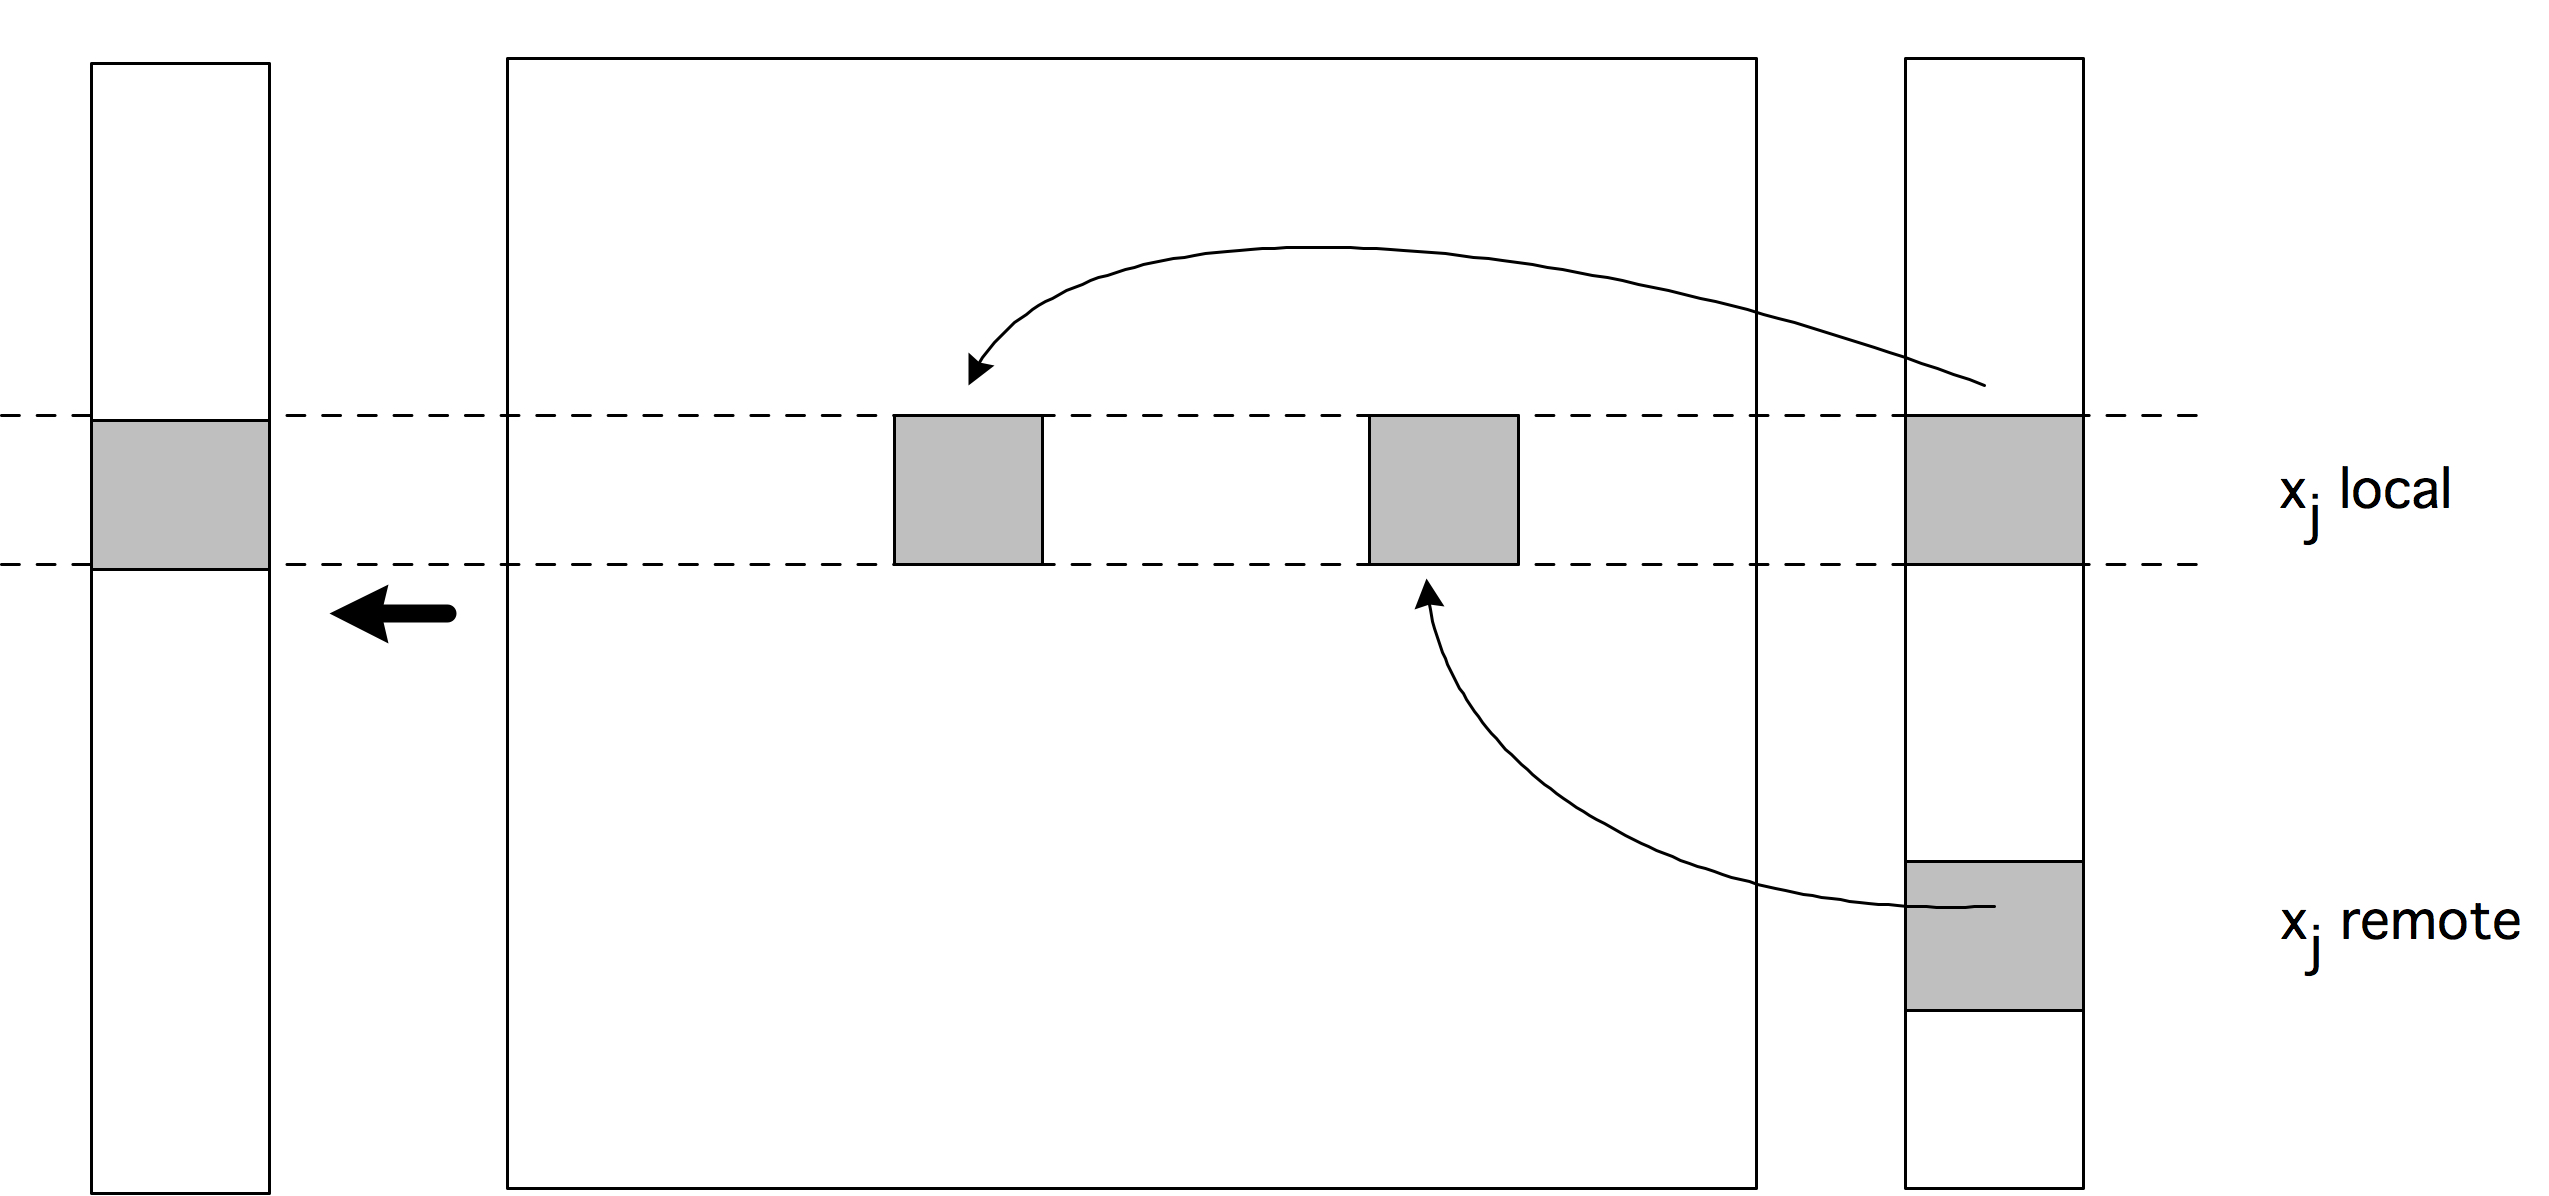
\includegraphics[scale=.06]{distmvp}\\
Note possible overlap communication and computation;\\
only used in the sparse case
}

\begin{frame}{Sparse matrix operations}
\begin{itemize}
\item Traditional: PDE, discussed next
\item New: graph algorithms and big data, discussed later
\end{itemize}
\end{frame}

\frame{\frametitle{Operator view of spmvp}
Difference stencil

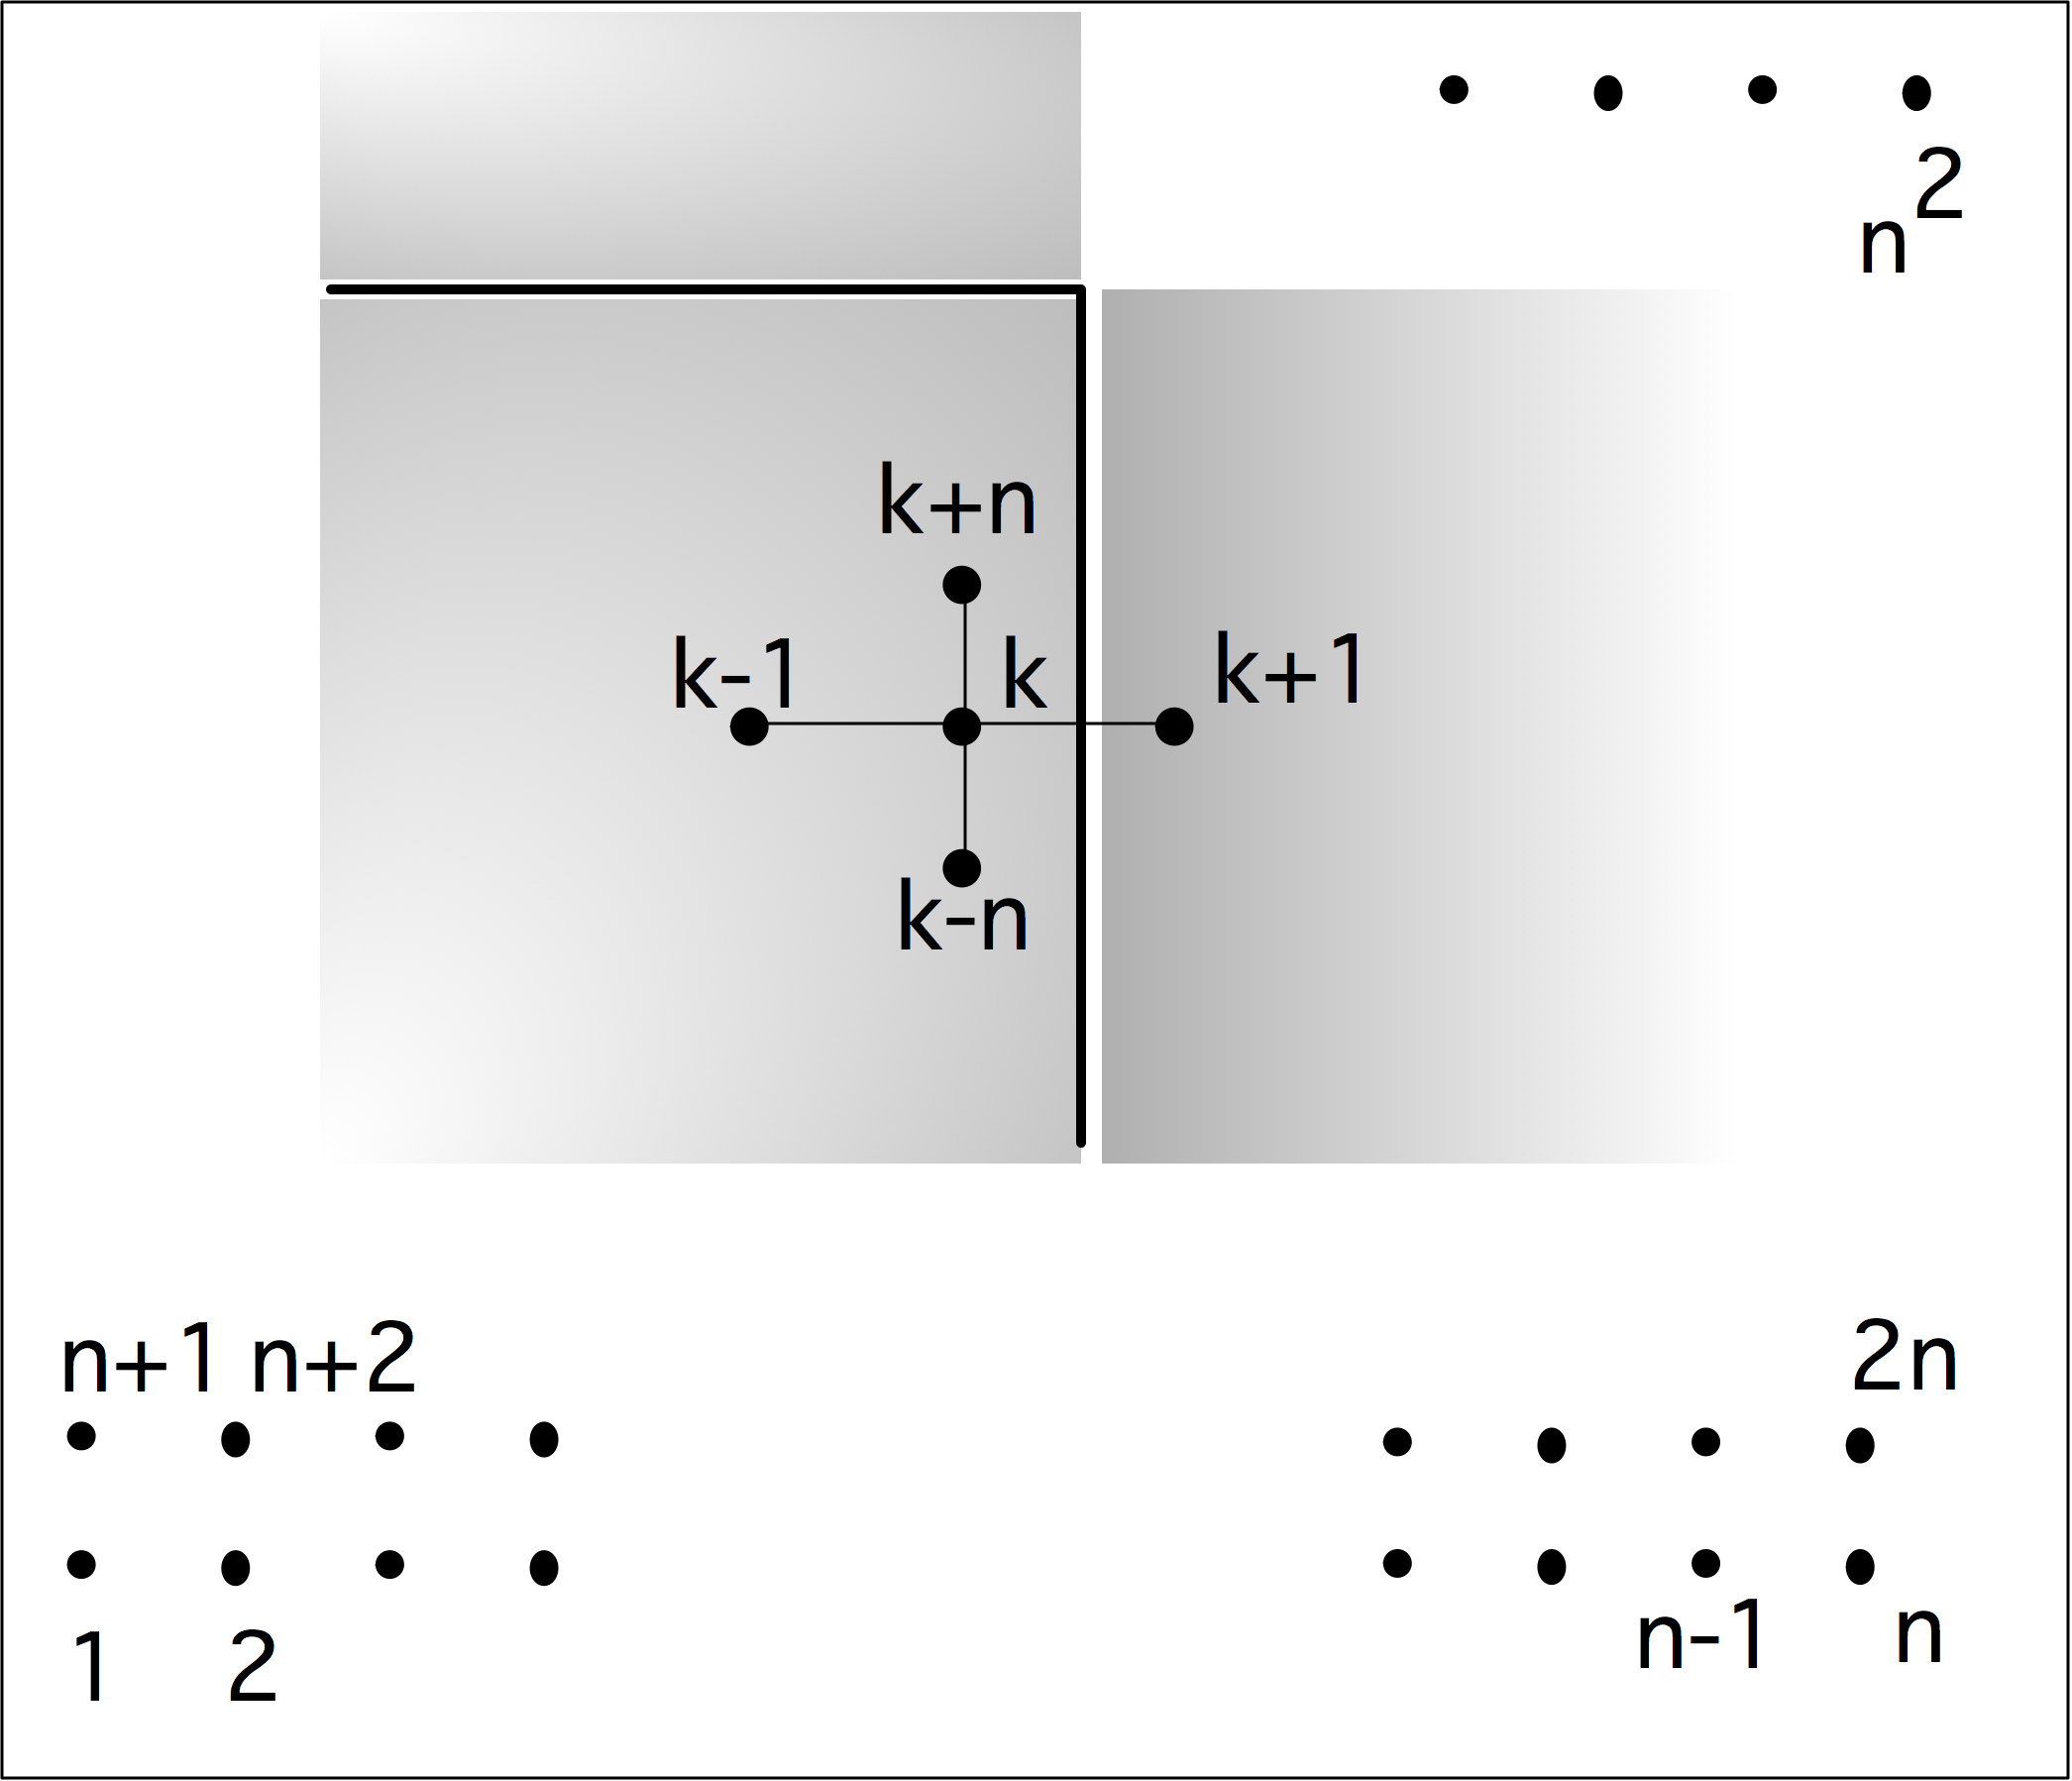
\includegraphics[scale=.09]{laplaceparallel}
}

\frame{\frametitle{Parallel operator view}
induces ghost region:

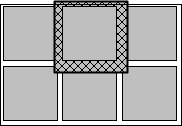
\includegraphics[scale=.5]{ghost}

Limited number of neighbours, limited buffer space
}

\begin{frame}{Matrix vs operator view}
\begin{itemize}
\item Domain partitioning: processor `owns' variable~$i$
\item owns all connections from $i$ to other~$j$s
\item $\Rightarrow$ processor owns whole matrix row
\item $\Rightarrow$ 1D partitioning of the matrix, always
\end{itemize}
\end{frame}

\begin{frame}
\footnotesize
\begin{equation}
  \label{eq:5starmatrix}
  A=
  \left(\begin{array}{ccccc|ccccc|cc}
    4&-1&&&\emptyset&-1&&&&\emptyset&\\ 
    -1&4&-1&&&&-1&&&&\\ 
    &\ddots&\ddots&\ddots&&&&\ddots&&\\ 
    &&\ddots&\ddots&-1&&&&\ddots&\\ 
    \emptyset&&&-1&4&\emptyset&&&&-1&\\ \hline
    -1&&&&\emptyset&4&-1&&&&-1\\
    &-1      &      &&&-1      &4       &-1      &&&&-1\\
    &\uparrow&\ddots&&&\uparrow&\uparrow&\uparrow&&  &&\uparrow\\
    &k-n     &      &&&k-1     &k       &k+1     &&-1&&k+n\\
    &&&&-1&&&&-1&4&&\\ \hline
    &        &      &&&\ddots  &        &        &&  &\ddots\\
  \end{array}\right)
\end{equation}
\end{frame}

\frame{\frametitle{Scaling}
\begin{itemize}
\item Same phenomenon as with dense matrix:
\item $n^2$ variables, memory needed is $cn^2/p$
\item 1D partitioning \emph{of domain} does not weakly scale
\begin{itemize}
\item Message size is one line: $n$
\item is $\sqrt p \sqrt M$, goes up with processors
\end{itemize}
\item 2D partitioning \emph{of domain} scales weakly. 
\begin{itemize}
\item message size $n/\sqrt p=\sqrt M$
\item constant in $M$
\end{itemize}
\end{itemize}
}

\begin{frame}{MPI implementation}
\begin{itemize}
\item Assume general communication structure:\\
  neighbour processors can not statically be determined
\item Assume no structural symmetry
\item For matrix-vector product:\\
  each processor issues send and receive requests
\item Problem: receives are easy, sends are hard
\item \indexterm{Inspector-executor}: one-time discovery of structure,\\
  followed by many executions
\end{itemize}
\end{frame}

\begin{frame}{Asymmetry in reasoning}
Say
\begin{itemize}
\item Processor owns row $i$, $a_{ij}\not=0$, processor does not own~$j$
\end{itemize}
  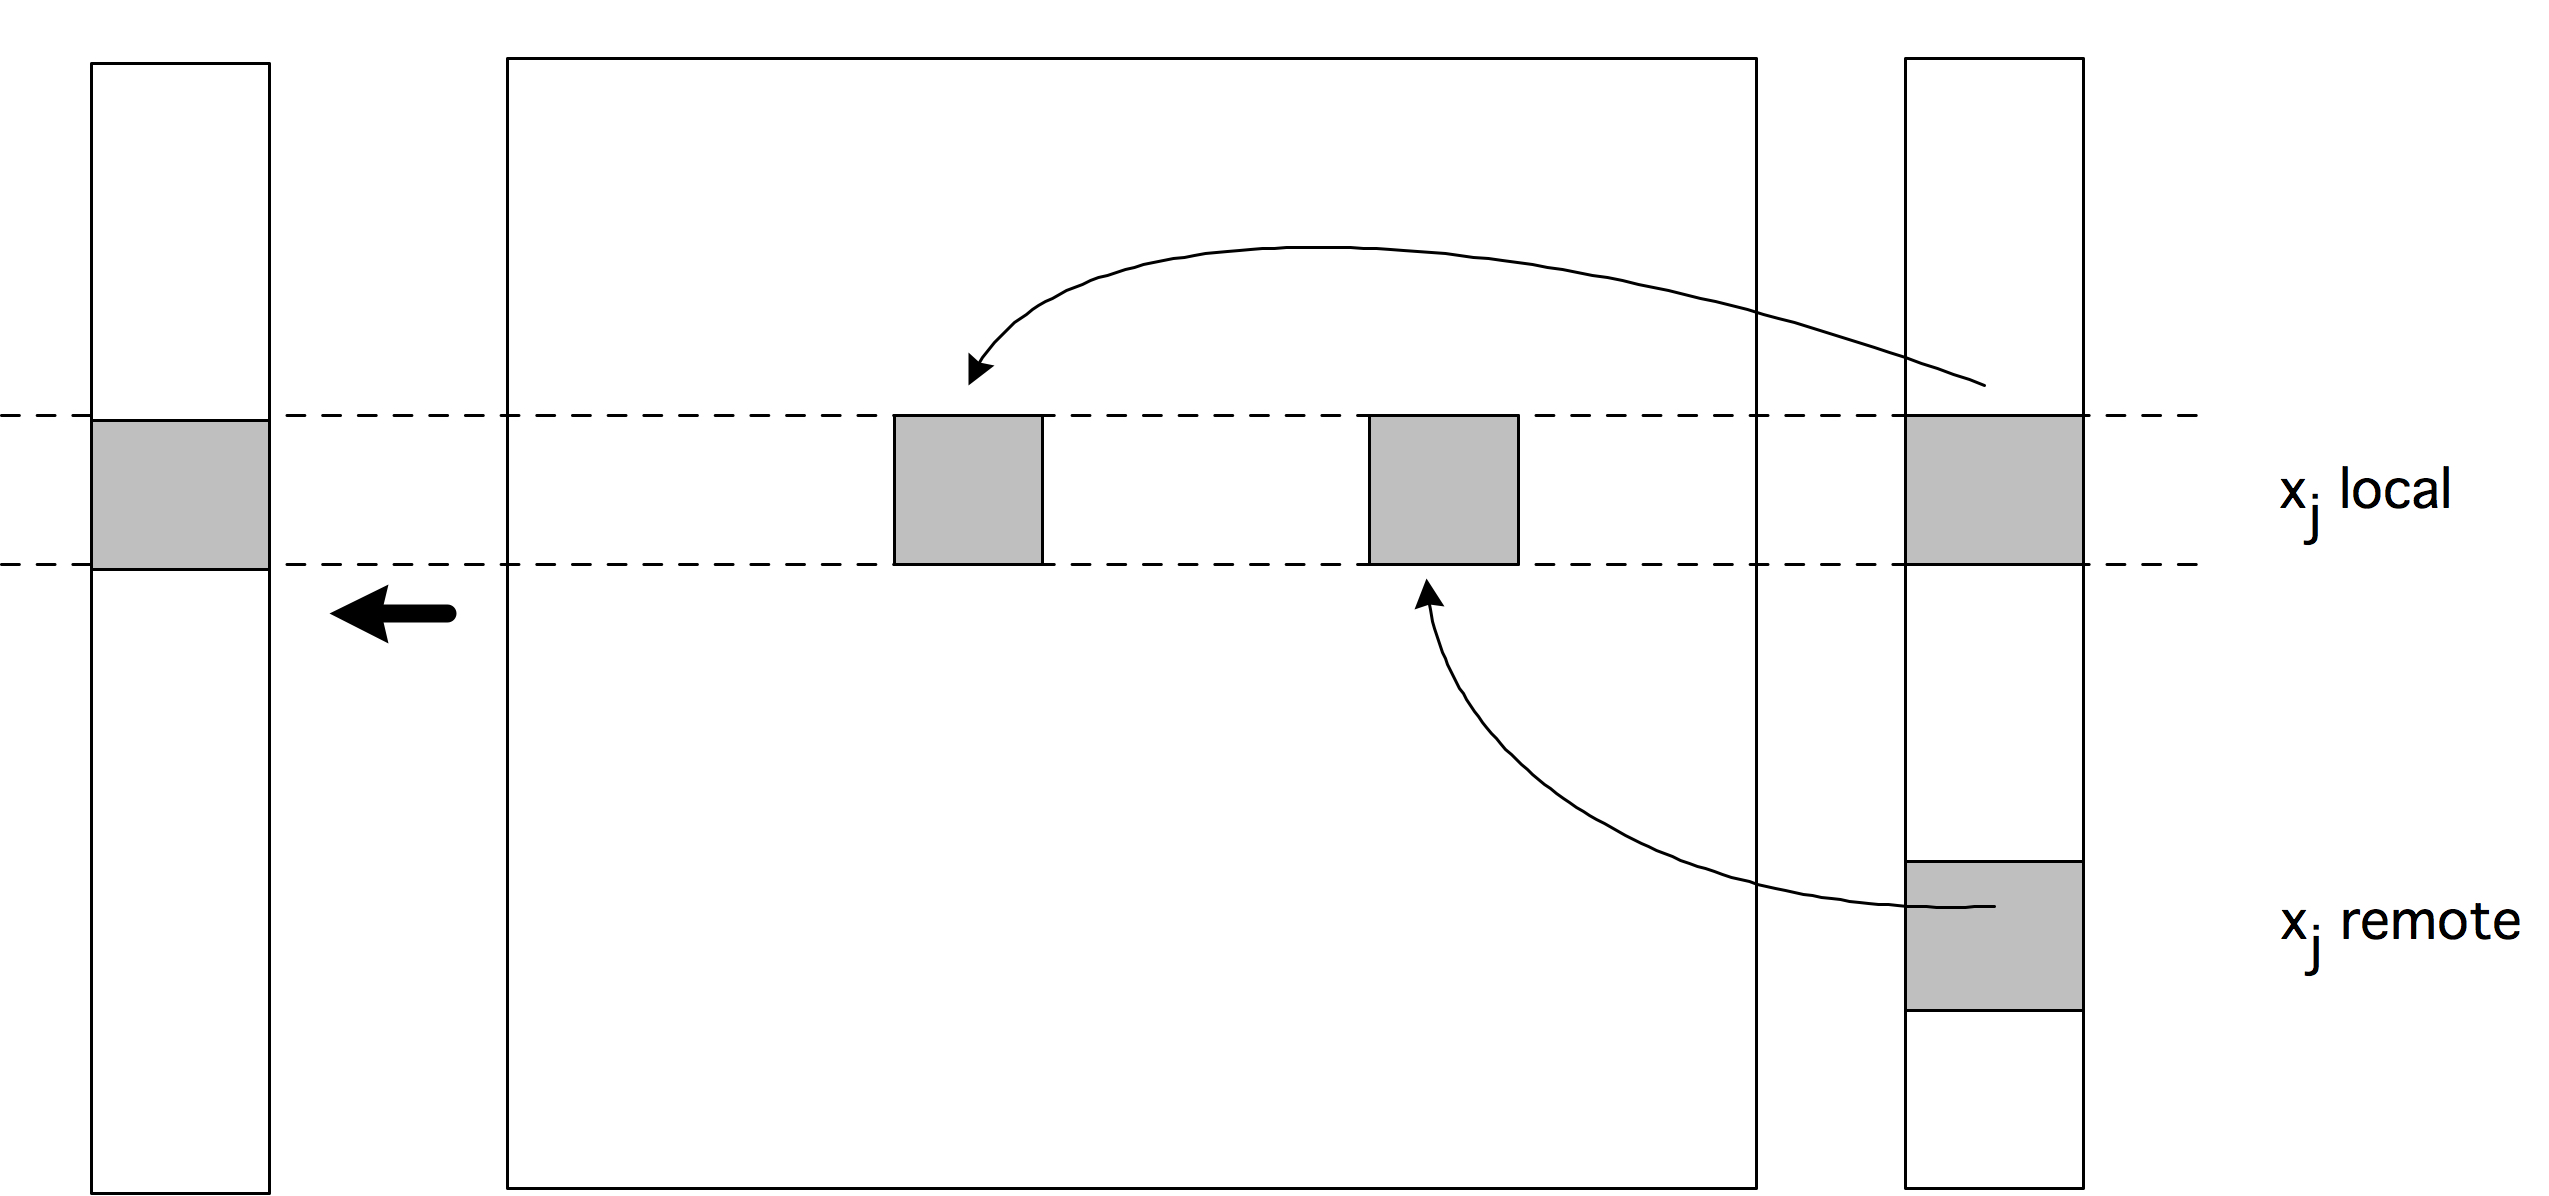
\includegraphics[scale=.06]{distmvp}\\
  \begin{itemize}
  \item Needed: message from $j$ to~$i$
  \item Processor $i$ can discover this
  \item Processor $j$ not in general
  \end{itemize}
\end{frame}

\begin{frame}{Reduce-scatter}
Make $p\times p$ matrix $C$:
\[ C_{ij}=
\begin{cases}
  1&\hbox{$i$ receives from $j$}\\ 0&\hbox{otherwise}
\end{cases}
\]
Then \[ s_j = \sum_i C_{ij} \]
number of messages sent by~$j$

Reduce-scatter, proc~$i$ has $C_{i*}$
\end{frame}

\begin{frame}{Reason for more cleverness}
  \begin{itemize}
  \item The above is collective, implies synchronization
  \item temp space $O(P)$
  \item can we get this down to $O(\#\mathrm{neighbours})$?
  \item \textsl{can we detect that we have received all requests\\
    without knowing how many to expect?}
  \end{itemize}
\end{frame}

\begin{frame}[fragile]{MPI 3 non-blocking barrier}
  \begin{itemize}
  \item Barrier: test that every process has reached this point\\
    blocking
  \item Ibarrier: non-blocking test
  \item Ibarrier calls does not block, yields \n{MPI_Request} pointer
  \item Use Wait or Test on the request
  \end{itemize}
\begin{verbatim}
  int MPI_Ibarrier(MPI_Comm comm, MPI_Request *request)
\end{verbatim}
\end{frame}

\begin{frame}[fragile]{DTD algorithms}
  `Distributed Termination Detection'\\
  used to be (extremely) tricky, now easy with MPI~3

  Establish sparse neighbours:
  \begin{itemize}
  \item Send all your own requests (Isend)
  \item Loop:
    \begin{itemize}
    \item Test on send requests; if all done, enter non-blocking barrier
    \item Probe for request messages, receive if there is something
    \item If you're in the barrier, also test for the barrier to complete
    \end{itemize}
  \item $\Rightarrow$ if the barrier completes, you have received all your requests
  \end{itemize}
  (For safety, use \n{MPI_Issend})
\end{frame}

